\chapter[METODOLOGIA]{METODOLOGIA}

Este capítulo descreve o conjunto de dados, a arquitetura do \textit{pipeline}, o protocolo de calibração, a regra que produz os limiares, a referência adotada para avaliação e o desenho dos dois experimentos.

\section{Caracterização da Pesquisa}

O trabalho classifica-se como pesquisa aplicada, de natureza experimental e abordagem predominantemente quantitativa. É aplicada porque endereça um problema concreto da indústria de rochas ornamentais. É experimental porque manipula variáveis controladas --- o escopo sobre o qual a regra de calibração é aplicada e a quantidade de modelos treinados --- e observa seu efeito sobre métricas de sobreposição com uma referência anotada.

\section{Conjunto de Dados}

O conjunto de imagens é público, obtido na plataforma Kaggle \cite{dataset_araujo2023}. O autor deste trabalho \textbf{não constituiu} o banco: selecionou, caracterizou e pré-processou um conjunto existente. Essa escolha tem uma consequência metodológica favorável --- todo o protocolo pode ser reproduzido por terceiros sem acordo com nenhuma empresa.

O conjunto reúne 34.630 imagens de chapas polidas, distribuídas em 45 litologias. O conjunto é distribuído já particionado, nas proporções de 70\%, 15\% e 15\% em todas as classes, com 24.263 imagens de treinamento, 5.214 de validação e 5.153 de teste. Este trabalho adota as partições originais sem alteração. A atribuição das imagens às partições, porém, \textbf{não é aleatória por imagem}: a numeração dos arquivos segue a sequência de corte das chapas, de modo que imagens consecutivas são chapas vizinhas do mesmo bloco, e em ao menos uma litologia a partição de teste aparenta vir de um bloco ausente do treinamento (Seção \ref{sec:res_classificador}).

Uma única alteração foi feita sobre o conjunto original: a pasta de uma litologia, grafada \textit{whte\_liberdade} na fonte, foi renomeada para \textit{white\_liberdade}. A correção não é apenas estética. O índice de classe é a posição do nome na ordem alfabética, e a grafia original deslocava sete classes; quem reproduzir o trabalho a partir da fonte pública precisa repetir a renomeação.

A distribuição entre litologias é fortemente desbalanceada, variando de 106 a 4.588 imagens. Em vez de equalizar artificialmente essa distribuição, o trabalho a converte em variável do experimento, agrupando as litologias em quatro faixas de volume, conforme o Quadro \ref{quad:faixas}.

\begin{quadro}[ht]
  \caption{Faixas de volume de dados e respectivo número de litologias.}
  \label{quad:faixas}
  \centering
  \begin{tabularx}{\textwidth}{clcX}
    \hline
    \bfseries Faixa & \bfseries Critério & \bfseries Litologias & \bfseries Observação \\
    \hline
    A & $\geq$ 1.000 imagens & 11 & Faixa de execução prioritária \\
    B & 500 a 999 imagens & 6 & \\
    C & 200 a 499 imagens & 14 & \\
    D & $<$ 200 imagens & 14 & Inclui as litologias de textura atípica \\
    \hline
  \end{tabularx}
  \legend{Fonte: elaborado pelo autor.}
\end{quadro}

A ordem de execução dos experimentos segue as faixas, da maior para a menor, e cada faixa constitui um marco entregável: ela é executada, avaliada e redigida antes que a seguinte comece. Em qualquer ponto de interrupção existe, assim, um resultado completo e reportável, e as faixas não alcançadas são declaradas como trabalho futuro.

\section{Arquitetura do \textit{Pipeline}}

O ARIA organiza-se em três estágios, descritos no Quadro \ref{quad:estagios}. O primeiro identifica a litologia da chapa e roteia; o segundo gera os polígonos de anomalia fora da linha de produção; o terceiro executa a inferência rápida em produção.

\begin{quadro}[ht]
  \caption{Estágios do \textit{pipeline} ARIA.}
  \label{quad:estagios}
  \centering
  \begin{tabularx}{\textwidth}{llX}
    \hline
    \bfseries Estágio & \bfseries Modelo & \bfseries Papel \\
    \hline
    1 --- Classificador & Xception (reprodução do DeepStoneAI) & Identifica a litologia e seleciona a configuração de sondas e o modelo Aluno correspondente \\
    2 --- Professor & Modelo de fundação guiado por texto & Gera polígonos de anomalia sem anotação humana, processando o conjunto fora de linha \\
    3 --- Aluno & YOLO11-seg & Executa a inferência em produção, treinado sobre os polígonos do Professor \\
    \hline
  \end{tabularx}
  \legend{Fonte: elaborado pelo autor.}
\end{quadro}

A separação entre Professor e Aluno é o que torna o arranjo viável industrialmente: o custo de inferência do modelo de fundação é pago uma única vez, na geração do conjunto de treinamento, e não a cada chapa inspecionada. A Figura \ref{fig:arquitetura} mostra o fluxo nas duas fases: fora da linha, a seleção de imagens, a calibração e o Professor produzem o conjunto de treinamento do Aluno; em produção, o classificador identifica a litologia e encaminha a chapa ao Aluno correspondente.

\begin{figure}[ht]
  \caption{Fluxo de processamento do \textit{pipeline} ARIA.}
  \label{fig:arquitetura}
  \centering
  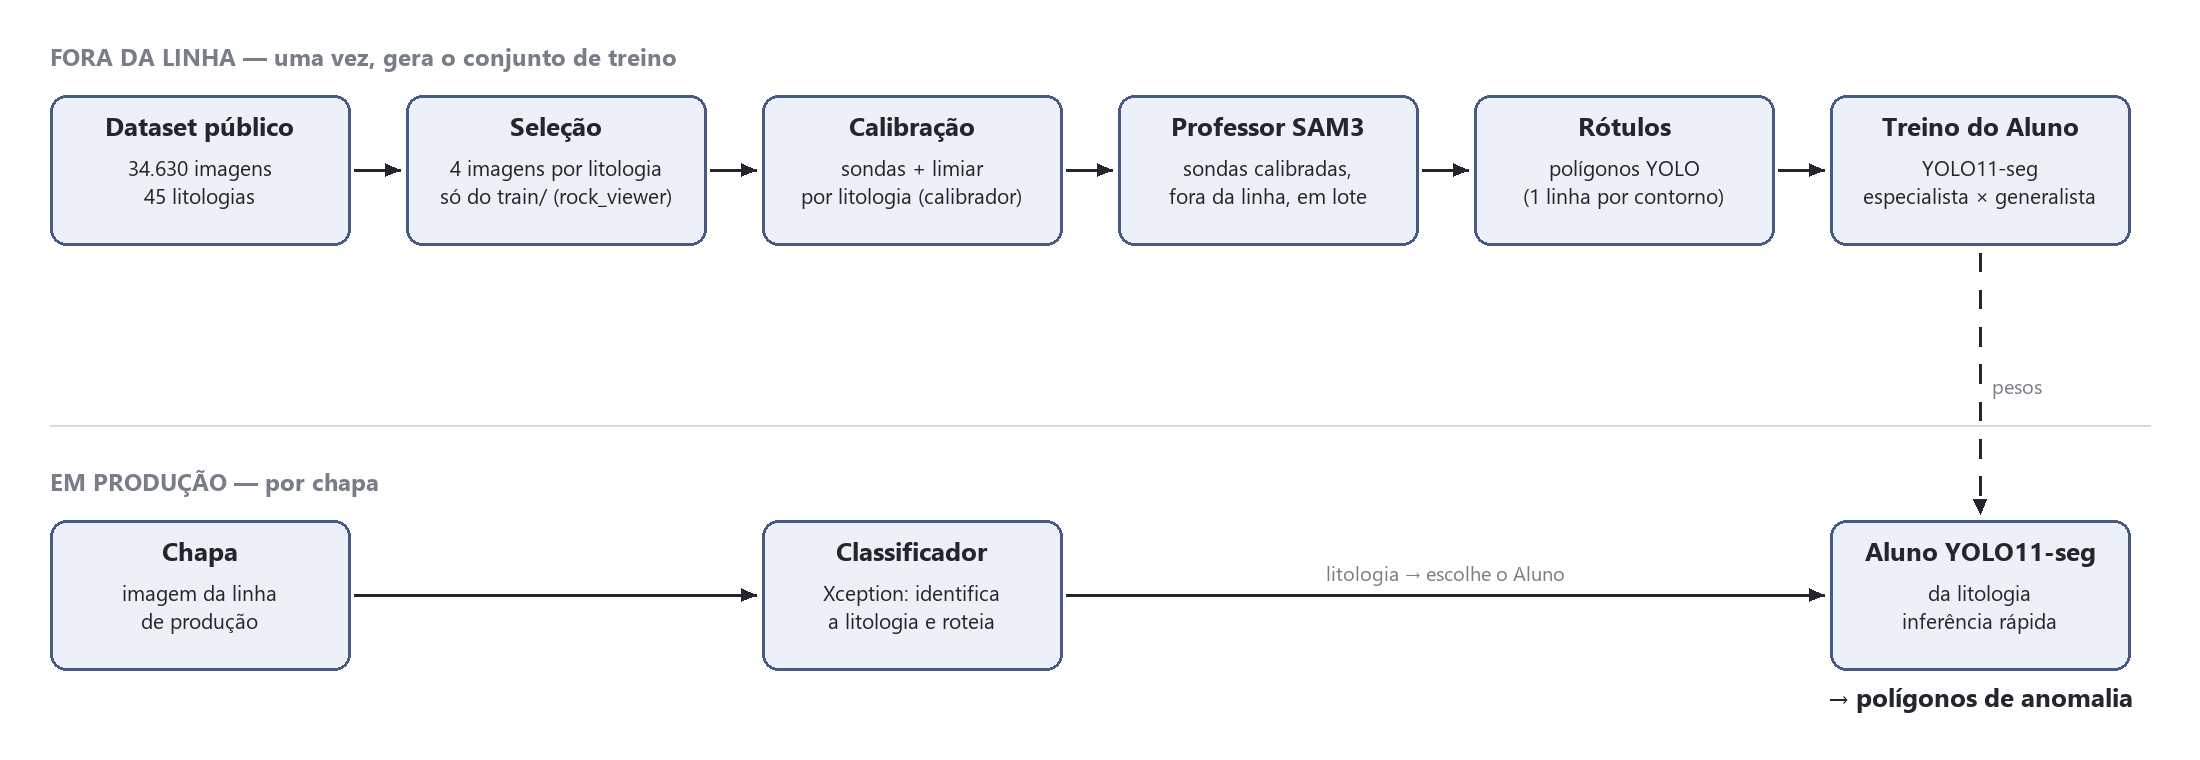
\includegraphics[width=\textwidth]{arquitetura_aria.png}
  \legend{Fonte: elaborado pelo autor.}
\end{figure}

\section{Estágio 1 --- Reprodução do Classificador de Litologias}
\label{sec:classificador}

O classificador do primeiro estágio é uma \textbf{reprodução} do modelo Xception do DeepStoneAI \cite{deepstoneai_moreira2025}, e não o modelo original: o material publicado daquele trabalho traz a receita de treinamento, em cadernos Keras, mas não os pesos treinados. A receita foi mantida --- pesos iniciais do ImageNet, 15 épocas com a base congelada e taxa de aprendizado de $10^{-4}$, ajuste fino das últimas 50 camadas com taxa de $10^{-5}$, aumento de dados por espelhamento, rotação, \textit{zoom} e contraste, e ausência de pesos por classe. Quatro aspectos foram alterados, conforme o Quadro \ref{quad:xception}.

\begin{quadro}[ht]
  \caption{Diferenças entre o classificador original e a reprodução adotada.}
  \label{quad:xception}
  \centering
  \begin{tabularx}{\textwidth}{lXX}
    \hline
    \bfseries Aspecto & \bfseries DeepStoneAI & \bfseries ARIA \\
    \hline
    Arcabouço     & Keras/TensorFlow & PyTorch, com a mesma arquitetura e os mesmos pesos iniciais \\
    Particionamento & Partições originais fundidas e sorteadas de novo por imagem & Partições originais do conjunto de dados, as mesmas da calibração \\
    Resolução     & Carregada em 480 e ampliada para 1.080 \textit{pixels} & 480 $\times$ 480 \textit{pixels}, sem ampliação \\
    Normalização  & Entrada em $[0, 1]$ & Entrada em $[-1, 1]$, a escala esperada pelos pesos do ImageNet \\
    \hline
  \end{tabularx}
  \legend{Fonte: elaborado pelo autor.}
\end{quadro}

A troca de arcabouço é de ordem prática. A alteração do particionamento é metodológica: com as partições originais, o classificador nunca é treinado sobre as imagens de teste das quais sai o conjunto de referência (Seção \ref{sec:referencia}). A correção da normalização ajusta a entrada à escala para a qual os pesos pré-treinados foram produzidos. A fidelidade da reprodução foi conferida no código, inclusive pela contagem de parâmetros treináveis na fase de ajuste fino, idêntica à do modelo original.

O classificador é avaliado uma única vez sobre a partição de teste, ao final do treinamento, por acurácia, acurácia balanceada e F1 macro.

\section{Sondas de Recall, não Rótulos Semânticos}
\label{sec:sondas}

O Professor é guiado por um conjunto de palavras em inglês, aqui denominadas \textbf{sondas}. O Quadro \ref{quad:sondas} lista o conjunto de trabalho e a assinatura visual que cada sonda costuma ativar.

\begin{quadro}[ht]
  \caption{Sondas textuais, identificadores e assinatura visual associada.}
  \label{quad:sondas}
  \centering
  \begin{tabularx}{\textwidth}{llX}
    \hline
    \bfseries Sonda & \bfseries \textit{id} & \bfseries Assinatura visual que costuma ativar \\
    \hline
    \textit{vein}         & 0 & Estrias e faixas contrastantes \\
    \textit{crack}        & 1 & Descontinuidades lineares finas e escuras \\
    \textit{Stain}        & 2 & Variação de cor em mancha difusa \\
    \textit{Dark patches} & 3 & Regiões escuras sobre fundo claro \\
    \textit{light spot}   & 4 & Regiões claras sobre fundo escuro \\
    \textit{scratch}      & 5 & Riscos superficiais finos \\
    \textit{white stain}  & 6 & Manchas brancas não marcadas por \textit{light spot} \\
    \hline
  \end{tabularx}
  \legend{Fonte: elaborado pelo autor.}
\end{quadro}

É necessário ser explícito quanto ao estatuto dessas palavras. Elas \textbf{não são afirmações sobre a natureza do que foi encontrado}: são chaves lexicais escolhidas por fazerem o modelo responder a certas assinaturas visuais. Afirmar que a região marcada pela sonda \textit{crack} \textit{é} uma fissura exigiria ter validado que o modelo distingue fissura de veio --- validação que este trabalho não realiza e, portanto, não pode alegar.

Dessa decisão decorre a \textbf{rotulagem binária}: todas as regiões marcadas recebem o mesmo identificador de classe no treinamento do Aluno. Os identificadores por sonda listados no Quadro \ref{quad:sondas} são preservados nos arquivos de anotação, para não perder o registro de qual sonda disparou cada região, mas são colapsados em uma única classe antes do treino. O objetivo do conjunto de sondas é maximizar a \textbf{cobertura} de regiões anômalas, não classificá-las. A rotulagem multiclasse fica registrada como trabalho futuro.

O conjunto de sondas não é fechado: ele pode crescer durante a calibração, sob uma condição. Qualquer palavra pode ser testada na ferramenta de calibração como sonda exploratória, com as máscaras exibidas, mas uma sonda só passa a gerar anotação depois de \textbf{registrada}, com identificador próprio --- e só é registrada quando marca regiões que nenhuma das sondas existentes marca. A sonda \textit{white stain} entrou dessa forma: testada sobre a litologia \textit{san\_francisco\_green}, marcou manchas brancas que \textit{light spot} não alcançava. O identificador de uma sonda é permanente, e sondas novas recebem o próximo número livre. Renumerar uma sonda já usada faria os arquivos de anotação gravados antes passarem a indicar outra sonda, sem erro algum que denunciasse a troca. Como os identificadores são colapsados em uma única classe antes do treino, registrar uma sonda a mais amplia a cobertura sem alterar a natureza do rótulo. Nas litologias calibradas antes do registro de uma sonda, ela permanece candidata não avaliada até que a litologia seja revista.

\section{Protocolo de Calibração}

Calibrar uma litologia significa responder a duas perguntas distintas: \textit{quais} sondas entram no conjunto, e com \textit{qual} limiar de confiança cada uma opera. A imagem ideal para responder a cada uma é oposta, e confundi-las é a origem de um viés concreto.

Para \textbf{descobrir} quais sondas respondem, a imagem deve conter o máximo de fenômenos --- quanto mais rica, melhor. Para \textbf{escolher} o limiar, a imagem deve representar a variação típica da litologia. Usar a chapa mais rica para as duas tarefas produz um efeito de seleção por visibilidade: as feições foram escolhidas justamente por serem visíveis, e o limiar resultante sai alto demais, perdendo o defeito sutil das demais chapas. Usar a chapa mais sutil produz o erro oposto --- limiar baixo e enxurrada de marcações na chapa comum.

O protocolo adotado separa as duas tarefas em quatro imagens por litologia, descritas no Quadro \ref{quad:vagas}.

\begin{quadro}[ht]
  \caption{As quatro imagens de calibração por litologia e o papel de cada uma.}
  \label{quad:vagas}
  \centering
  \begin{tabularx}{\textwidth}{llX}
    \hline
    \bfseries Imagem & \bfseries Decide & \bfseries Critério de seleção \\
    \hline
    \textit{descoberta}    & Quais sondas entram & A chapa com o maior número de tipos distintos de feição \\
    \textit{limiar sutil}  & O limiar & Feições fracas, de baixo contraste \\
    \textit{limiar típica} & O limiar & A chapa mais comum da litologia \\
    \textit{limiar forte}  & O limiar & Feições marcantes, de alto contraste \\
    \hline
  \end{tabularx}
  \legend{Fonte: elaborado pelo autor.}
\end{quadro}

Três observações completam o protocolo.

Primeiro, as três imagens de limiar \textbf{não produzem três limiares a serem promediados}. Trata-se de um único limiar submetido a três casos. A média de três ótimos não é um ótimo: o caso sutil pediria um valor baixo, o caso forte um valor alto, e a média seria um número nunca verificado em imagem alguma, possivelmente ruim nas duas pontas. A pergunta deixa de ser "qual limiar acerta esta imagem", que não tem resposta, e passa a ser "qual limiar menos erra nas três", que tem.

Segundo, a seleção das quatro imagens é \textbf{manual}. Usar o próprio Professor para escolher as imagens de calibração seria raciocínio circular.

Terceiro, as quatro imagens saem exclusivamente da partição de \textbf{treinamento}. O conjunto de referência da avaliação sai da partição de teste, e calibrar sobre uma imagem de teste equivaleria a ajustar o limiar sobre a própria prova. A restrição tem um custo, que se declara: como as partições não são sorteadas por imagem, um fenômeno presente apenas em um bloco que caiu inteiro na partição de teste não pode ser visto durante a calibração. Esse custo é também o que torna a avaliação mais exigente --- o conjunto de referência mede a marcação inclusive em chapas que a calibração não teve como antecipar. Para as litologias da faixa A, a partição de treinamento reúne de 700 a 3.200 imagens, e o que limita a cobertura na escolha das imagens de calibração é a varredura do autor, não o tamanho da partição.

A origem de cada imagem selecionada --- partição e arquivo --- é registrada em um arquivo de metadados por litologia, compondo o material de reprodutibilidade do trabalho.

\subsection{Litologias movimentadas}

Durante a seleção das imagens da faixa A, o autor encontrou litologias de padrão movimentado, em que é difícil distinguir o que é defeito do que é o próprio desenho da pedra: o padrão natural já contém manchas, veios e contrastes fortes, e uma mesma feição pode valorizar a chapa ou desqualificá-la. Quatro litologias foram assim percebidas --- \textit{shadow\_white}, \textit{san\_francisco\_green}, \textit{white\_mirage} e \textit{golden\_storm}. A lista é percepção do autor: nenhuma delas teve a classificação petrográfica confirmada.

Essas litologias são calibradas pelo mesmo protocolo das demais. Excluí-las retiraria quatro das onze litologias da faixa A e exigiria um critério de exclusão que não existe por escrito --- o que reproduziria, na seleção do experimento, o problema que o trabalho aponta na inspeção. A dificuldade de julgá-las também não é um desvio do trabalho: é a arbitrariedade da fronteira entre feição e defeito no seu caso mais forte. A opinião de um especialista do setor foi solicitada e não havia sido obtida quando a seleção foi feita, de modo que o julgamento do autor é, nessas quatro litologias, o elo mais frágil da calibração, e o registro de calibração de cada uma o declara.

O termo adotado é \textbf{movimentada}, em oposição a homogênea: designa a rocha cuja estrutura forma desenho, como bandamento ou foliação \cite{TODO-movimentada}. O termo ``exótica'', que circula no setor, foi evitado por designar uma categoria comercial, ligada a raridade e preço, que não descreve a dificuldade observada.

\section{A Regra que Produz o Limiar}
\label{sec:regra}

A escolha do limiar precisa ser governada por uma regra escrita. Selecionar o valor "no olho", ainda que por um observador experiente, reproduziria exatamente a prática que o Capítulo 1 aponta como problema --- com a diferença de que o observador passaria a ser o autor, em vez do inspetor.

Estabelece-se, portanto, a seguinte distinção, que é o núcleo do desenho:

\begin{description}
  \item[O valor do limiar] \textbf{muda} por litologia. É o objetivo da calibração.
  \item[A regra que produz o valor] \textbf{não muda}. É idêntica para todas as 45 litologias.
\end{description}

A regra adotada é a seguinte. Para cada sonda, constrói-se a curva que relaciona o limiar ao número de regiões marcadas, somando as três imagens de limiar da litologia. O limiar escolhido é o \textbf{joelho} dessa curva, definido como o ponto de máxima distância à corda que liga seus dois extremos, após normalização dos eixos \cite{kneedle_satopaa2011}.

Formalmente, seja $V = \{\text{sutil}, \text{típica}, \text{forte}\}$ o conjunto das imagens de limiar de uma litologia e $D_v$ o conjunto das detecções de uma sonda na imagem $v$, obtidas com o limiar no piso, cada detecção $d$ com escore $s_d$. A curva da regra é dada pela Equação \ref{eq:curva}:

\begin{equation}
  N(t) = \sum_{v \in V} \left| \{\, d \in D_v : s_d > t \,\} \right|
  \label{eq:curva}
\end{equation}

\noindent avaliada em uma grade de 80 limiares $t_1 < t_2 < \dots < t_n$ em progressão geométrica, entre 0,9 vez o menor e o maior escore observado nas três imagens. Os dois eixos são normalizados no intervalo $[0, 1]$, o do limiar em escala logarítmica:

\begin{equation}
  x_i = \frac{\ln t_i - \ln t_1}{\ln t_n - \ln t_1}, \qquad
  y_i = \frac{N(t_i) - \min_j N(t_j)}{\max_j N(t_j) - \min_j N(t_j)}
  \label{eq:normalizacao}
\end{equation}

\noindent Como $N$ é decrescente, os extremos normalizados são $(0, 1)$ e $(1, 0)$, e a corda que os liga é a reta $x + y - 1 = 0$. O limiar da regra é o ponto da grade mais distante dessa corda (Equação \ref{eq:joelho}):

\begin{equation}
  t^{*} = t_{i^{*}}, \qquad
  i^{*} = \arg\max_{i} \frac{\left| x_i + y_i - 1 \right|}{\sqrt{2}}
  \label{eq:joelho}
\end{equation}

A forma da regra foi escolhida entre duas alternativas. A outra fixaria o limiar como o maior valor que ainda marca uma fração mínima das feições anotadas nas imagens de limiar. Seria uma regra mais próxima do objetivo final, por medir acerto em vez de forma de curva, mas exigiria anotar manualmente as três imagens de limiar de cada litologia --- 135 imagens, quase o triplo do conjunto de referência inteiro (Seção \ref{sec:referencia}) --- e ainda introduziria um parâmetro livre, a fração mínima. O joelho dispensa anotação e não tem parâmetro a fixar. Sua adequação é verificada sem custo adicional, pelo mesmo conjunto de referência que avalia os experimentos.

Três aspectos da regra são fixados deliberadamente. A imagem de \textit{descoberta} \textbf{não} entra no cálculo: escolhida por ser a mais rica em feições, ela puxaria o limiar para cima, reintroduzindo o viés de seleção por visibilidade que o protocolo existe para evitar. O eixo do limiar é tomado em escala \textbf{logarítmica}, porque os escores concentram-se na década baixa --- medidos entre 0,011 e 0,770 em uma litologia de referência, com mediana entre 0,040 e 0,080 --- e, em escala linear, o joelho recairia sistematicamente sobre o primeiro ponto da curva. Por fim, a regra \textbf{não possui parâmetro livre}: não há constante a ser fixada por inspeção, o que elimina a possibilidade de ajustá-la para favorecer um resultado.

A regra é aplicada mecanicamente. Reconhece-se, porém, que uma curva pode enganar em casos particulares, e o autor pode divergir do valor produzido. Para que essa divergência não se torne invisível, a ferramenta de calibração registra \textbf{ambos} os valores --- o produzido pela regra e o adotado pelo autor --- junto de uma justificativa textual obrigatória. Na litologia \textit{siena\_white}, por exemplo, o critério registrado foi: ``Subi até o ponto em que a vaga típica para de marcar matriz limpa, aceitando perder feições mais fracas da vaga sutil; a vaga forte continua com todas as óbvias.'' A justificativa nomeia o que foi aceito perder, e é isso que a torna auditável: outra pessoa pode discordar do limiar sabendo exatamente que troca foi feita. Os dois valores têm papéis distintos no Experimento 1: o da regra alimenta os braços que testam a regra, e o adotado pelo autor ocupa um braço próprio, que mede o efeito do ajuste humano (Seção \ref{sec:exp1}). O valor adotado pelo autor é também o que rotula o conjunto de treinamento do Aluno, e deixá-lo fora do experimento significaria avaliar uma configuração que o sistema não usa. A taxa de concordância entre regra e autor é reportada como resultado à parte, e constitui evidência sobre a adequação da própria regra.

\section{Varredura de Limiares Fora de Linha}
\label{sec:varredura}

Calibrar exige comparar muitos limiares. Feito de modo ingênuo --- escolher um valor, executar o Professor, observar, ajustar e reexecutar --- cada iteração custa minutos de processamento em GPU, o que inviabiliza o protocolo da seção anterior em tempo humano.

A inspeção do código do arcabouço utilizado mostra que o limiar de confiança é aplicado como \textbf{filtro posterior} à inferência. O modelo produz máscaras e escores sem conhecimento do limiar; este apenas descarta as detecções cujo escore não o ultrapassa. A supressão de não-máximos ocorre depois do filtro, mas processa as detecções em ordem decrescente de escore e só remove uma detecção usando outra de escore \textbf{maior} --- de onde se conclui que incluir detecções de escore baixo não altera as decisões tomadas sobre as de escore alto.

Segue-se que executar o Professor uma única vez com o limiar no piso, armazenar escores e polígonos, e filtrar esse material posteriormente é \textbf{exatamente equivalente} a reexecutar o modelo em cada limiar --- não se trata de aproximação. O ciclo de calibração passa de minutos por iteração a milissegundos, e é o que torna viável exibir simultaneamente o efeito de um mesmo limiar sobre as quatro imagens da litologia.

A equivalência não foi assumida: ela é verificada experimentalmente, e o procedimento de verificação é descrito na Seção \ref{sec:verificacao} e seu resultado reportado no Capítulo 4.

\section{Ferramentas de Seleção e Calibração}
\label{sec:ferramentas}

O protocolo das seções anteriores é executado com duas ferramentas desenvolvidas para este trabalho e mantidas no repositório. As responsabilidades são separadas de propósito: a ferramenta de seleção apenas escolhe as quatro imagens de cada litologia; a de calibração apenas decide quais sondas entram e com que limiar; e somente o \textit{script} de inferência do Professor grava as anotações finais. Nenhuma das duas primeiras produz rótulo de treinamento.

\subsection{Seleção das imagens}

A ferramenta de seleção exibe, no navegador, a grade de todas as imagens da partição de treinamento de uma litologia, conforme a Figura \ref{fig:rock_viewer}. O cabeçalho mostra a faixa de volume, o total de imagens, as quatro vagas com seu estado e a instrução da vaga em preenchimento --- para a vaga de descoberta, por exemplo, a de procurar a chapa com o maior número de tipos distintos de feição. Cada imagem pode ser ampliada e percorrida pelo teclado, e a escolha é confirmada digitando-se seu número.

\begin{figure}[ht]
  \caption{Ferramenta de seleção: grade de imagens de uma litologia, com as quatro vagas e a instrução da vaga em preenchimento.}
  \label{fig:rock_viewer}
  \centering
  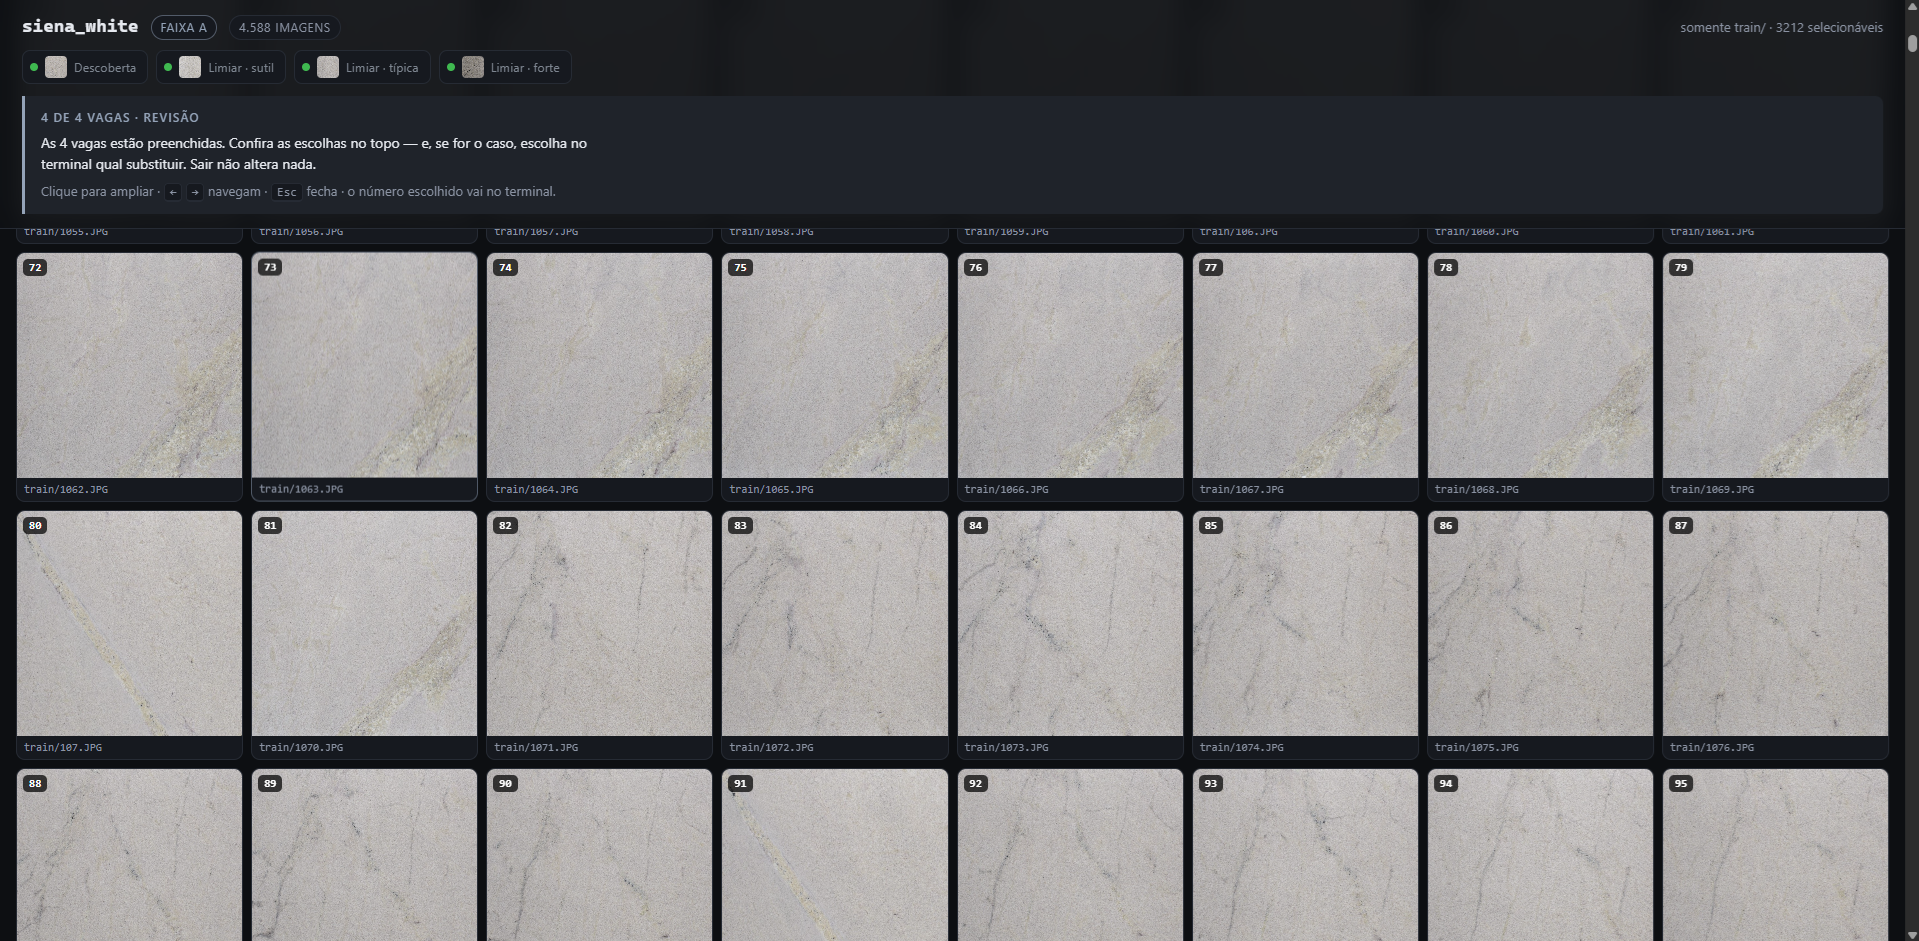
\includegraphics[width=\textwidth]{rock_viewer.png}
  \legend{Fonte: elaborado pelo autor.}
\end{figure}

Três propriedades do protocolo são garantidas pela ferramenta, e não pela disciplina de quem a opera. Somente imagens da partição de treinamento podem ser escolhidas; as das demais partições podem ser exibidas para estudo da variabilidade da rocha, mas aparecem bloqueadas e são recusadas. As litologias são oferecidas em ordem de volume de dados, da faixa A para a D, de modo que a ordem de trabalho é a própria prioridade do experimento. E cada escolha é copiada para um arquivo nomeado pelo papel da vaga, com a partição, o arquivo de origem e a data registrados nos metadados da litologia.

\subsection{Calibração}

A ferramenta de calibração é uma aplicação web local organizada em três etapas, que correspondem às duas perguntas da Seção \ref{sec:regra} e ao registro da resposta. A única etapa que usa a GPU é a captura: o Professor é executado com o limiar no piso sobre cada par (imagem, sonda) ainda sem material armazenado. Tudo o que vem depois opera sobre esse material, pela equivalência da Seção \ref{sec:varredura}.

Na etapa de \textbf{descoberta} (Figura \ref{fig:calib_descoberta}), cada sonda candidata é exibida sobre a imagem de descoberta, com o número de detecções e a faixa de escores. O limiar usado nessa tela serve apenas para visualizar e não é gravado: a pergunta é se a sonda responde a algo que existe na rocha, e não onde cortá-la. O autor marca as sondas que entram no conjunto; sondas exploratórias ainda não registradas podem ser vistas, mas não marcadas.

\begin{figure}[ht]
  \caption{Calibração, etapa de descoberta: as sondas candidatas sobre a imagem de descoberta.}
  \label{fig:calib_descoberta}
  \centering
  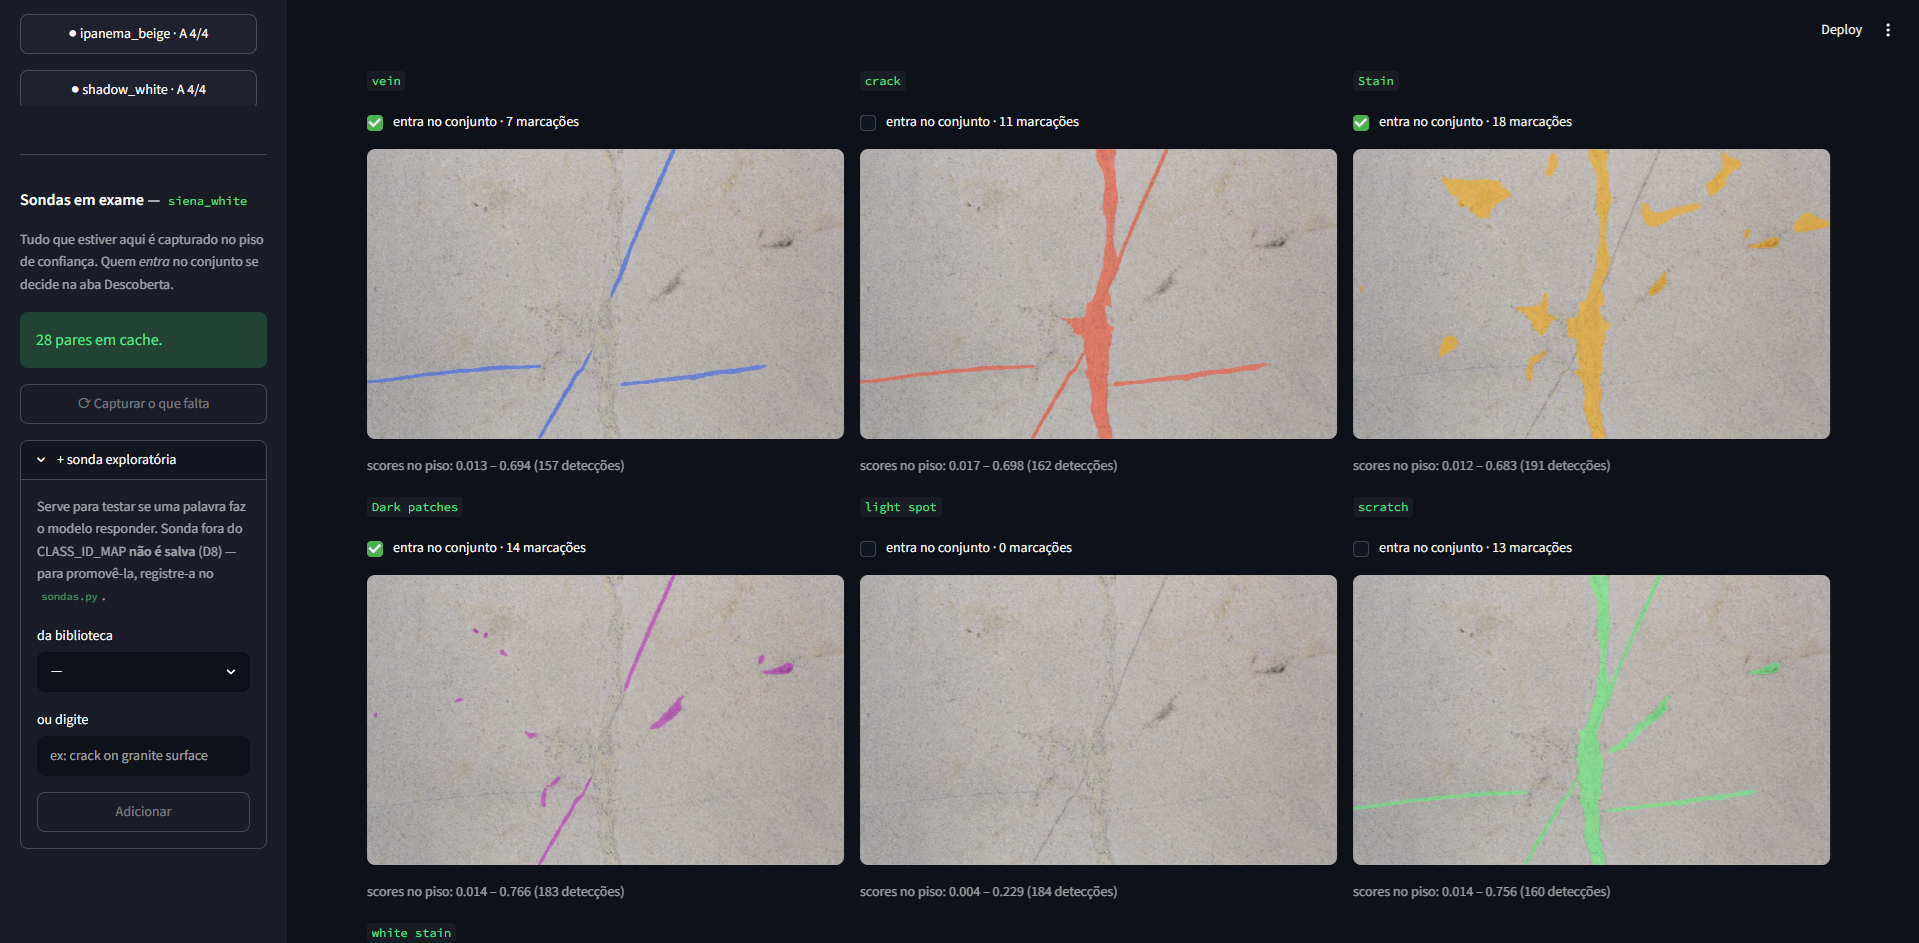
\includegraphics[width=\textwidth]{calib_descoberta.png}
  \legend{Fonte: elaborado pelo autor.}
\end{figure}

Na etapa de \textbf{limiar} (Figura \ref{fig:calib_limiar}), um único controle de limiar por sonda governa quatro prévias simultâneas, uma por imagem, cada uma com sua contagem de marcações. É a forma visual do princípio da Seção \ref{sec:regra}: um limiar submetido a três casos, e não três limiares a serem combinados. Abaixo das prévias, a curva da Equação \ref{eq:curva} é traçada por imagem, em escala logarítmica, com o limiar corrente e o limiar da regra marcados. O controle parte do valor da regra; o autor diverge dele se quiser, e nunca o contrário.

\begin{figure}[ht]
  \caption{Calibração, etapa de limiar: um controle, quatro prévias simultâneas e a curva com o limiar da regra marcado.}
  \label{fig:calib_limiar}
  \centering
  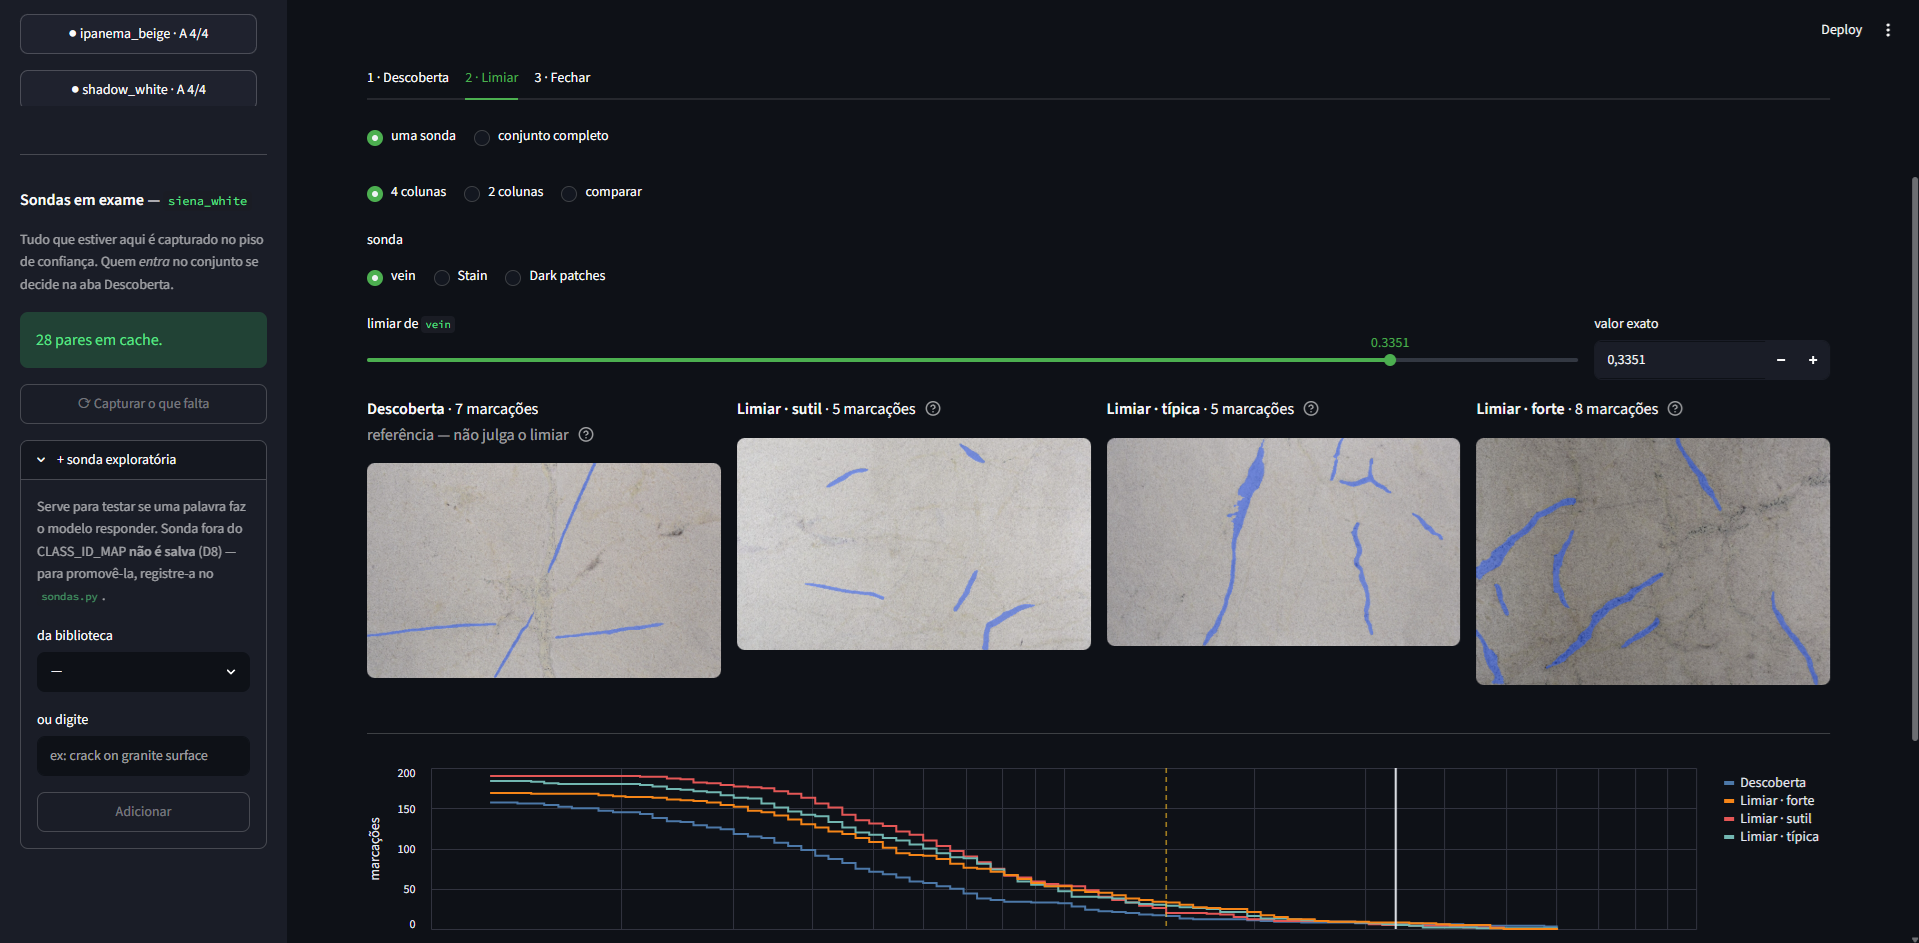
\includegraphics[width=\textwidth]{calib_limiar.png}
  \legend{Fonte: elaborado pelo autor.}
\end{figure}

Na etapa de \textbf{fechamento} (Figura \ref{fig:calib_fechar}), uma tabela reúne, por sonda, o limiar da regra, o adotado pelo autor, a divergência entre os dois e as marcações em cada imagem. O salvamento permanece bloqueado enquanto o campo do critério estiver vazio: não é possível gravar um limiar sem escrever por que ele foi escolhido.

\begin{figure}[ht]
  \caption{Calibração, etapa de fechamento: regra, limiar do autor e divergência por sonda, e o campo obrigatório do critério.}
  \label{fig:calib_fechar}
  \centering
  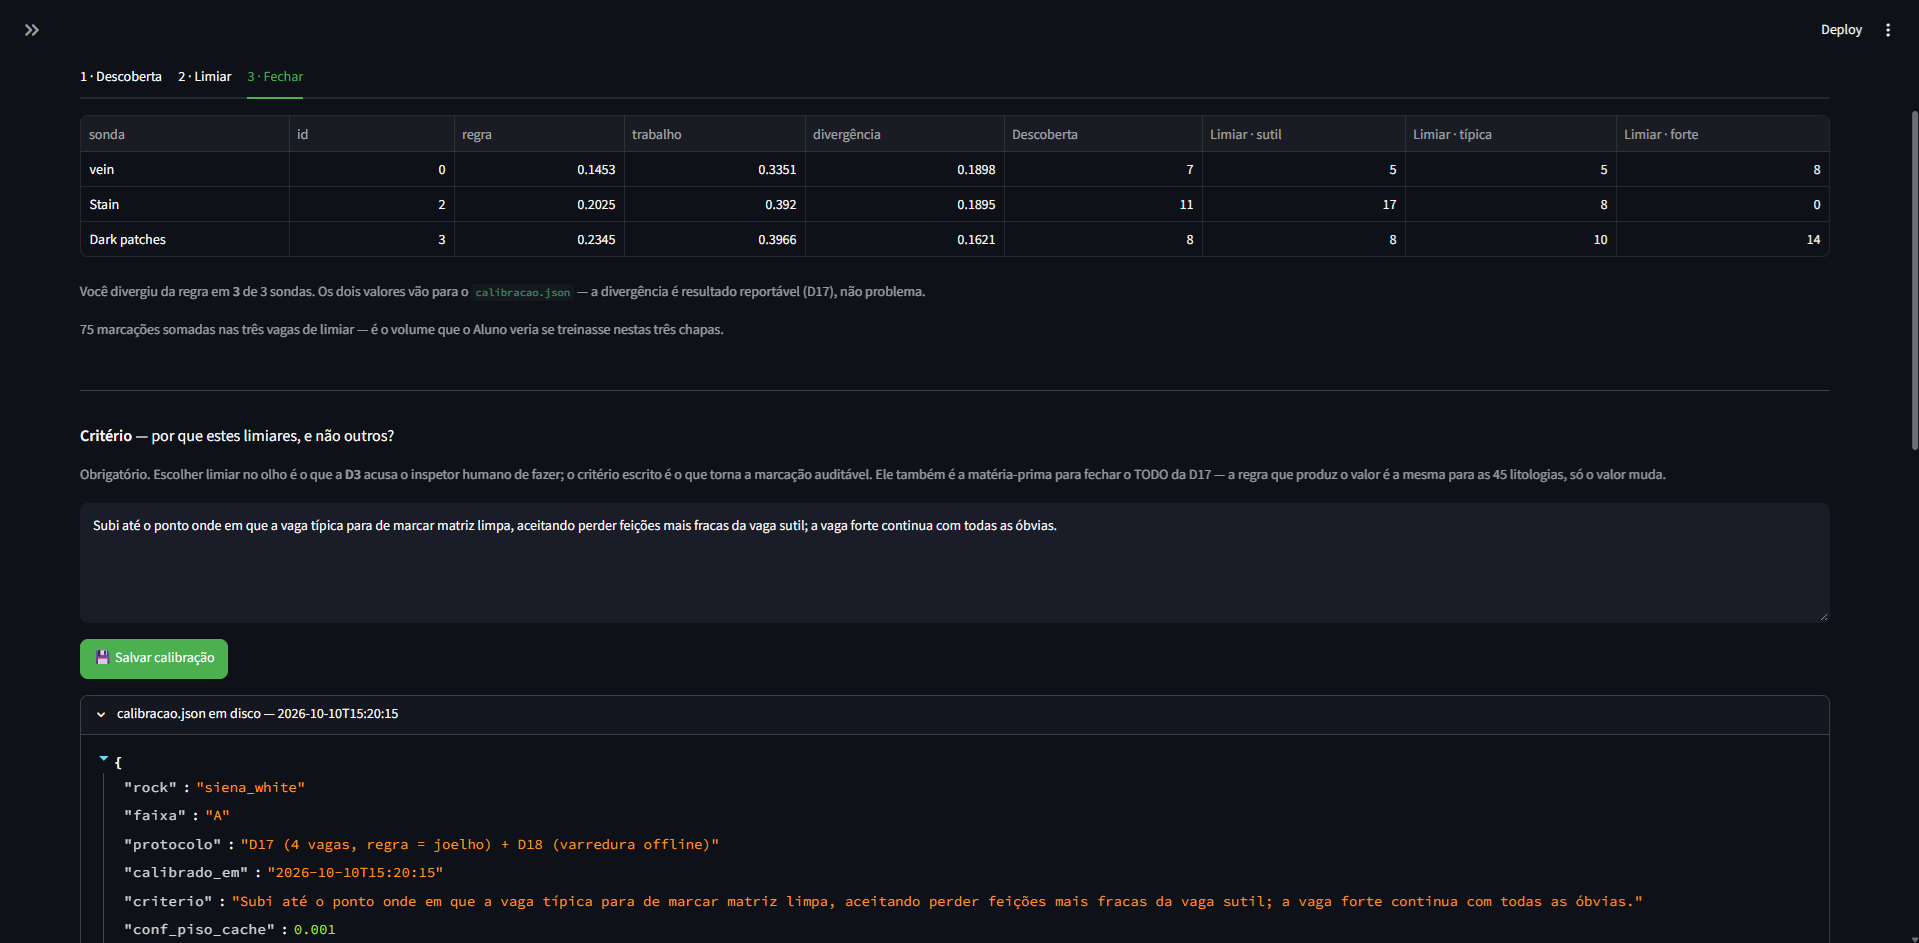
\includegraphics[width=\textwidth]{calib_fechar.png}
  \legend{Fonte: elaborado pelo autor.}
\end{figure}

\subsection{O registro de calibração}

O salvamento produz o registro de calibração da litologia, um arquivo de texto versionado junto do código. O Código \ref{lst:calibracao} mostra um trecho do registro da \textit{siena\_white}, com uma das três sondas do conjunto.

\begin{lstlisting}[caption={Trecho do registro de calibração da litologia \textit{siena\_white}.}, label={lst:calibracao}, literate={á}{{\'a}}1 {é}{{\'e}}1 {í}{{\'i}}1 {ó}{{\'o}}1 {ú}{{\'u}}1 {ã}{{\~a}}1 {õ}{{\~o}}1 {ç}{{\c{c}}}1 {â}{{\^a}}1 {ê}{{\^e}}1 {ô}{{\^o}}1]
{
  "rock": "siena_white",
  "faixa": "A",
  "protocolo": "D17 (4 vagas, regra = joelho) + D18 (varredura offline)",
  "calibrado_em": "2026-10-10T15:20:15",
  "criterio": "Subi até o ponto [...]",
  "conf_piso_cache": 0.001,
  "ultralytics": "8.4.61",
  "sondas_na_regra": 0,
  "sondas_divergentes": ["vein", "Stain", "Dark patches"],
  "sondas": {
    "vein": {
      "limiar_trabalho": 0.3351,
      "limiar_regra": 0.1453,
      "divergencia": 0.1898,
      "marcacoes_por_vaga": {
        "descoberta": 7, "limiar_sutil": 5,
        "limiar_tipica": 5, "limiar_forte": 8
      }
    }
  }
}
\end{lstlisting}

Cada campo responde a uma pergunta que um auditor faria. O critério diz por que o limiar é aquele. Os dois limiares e a divergência dizem quanto do valor veio da regra e quanto do autor. As contagens por imagem permitem conferir o efeito do limiar sem reexecutar nada. O piso e a versão da biblioteca dizem sob que condições a varredura fora de linha foi exata. É esse arquivo, e não o modelo treinado, que materializa a contribuição do trabalho: o critério de marcação de uma litologia, escrito em um lugar onde pode ser lido, contestado e versionado.

\section{Referência de Avaliação}
\label{sec:referencia}

Toda métrica quantitativa de segmentação exige uma referência. Usar a saída do próprio Professor como referência mediria fidelidade de cópia, não acerto, e tornaria a comparação entre braços experimentais destituída de sentido --- cada braço teria um gabarito diferente. Adotam-se, portanto, duas fontes de referência complementares.

\subsection{Conjunto de referência anotado}

Constitui-se um conjunto de aproximadamente 50 imagens, retiradas da partição de \textbf{teste} e distribuídas entre litologias da faixa A. Essas imagens são anotadas manualmente pelo autor \textbf{antes} de qualquer inferência ser executada sobre elas. A ordem é parte da metodologia: anotar depois de ver a máscara do modelo ancora o anotador nela, e a anotação deixa de ser independente.

É preciso delimitar o que essa precaução garante e o que não garante. Ela garante que a anotação não é cópia da máscara do modelo. Ela \textbf{não} garante neutralidade: o autor desenvolveu o protocolo de calibração observando saídas do Professor durante meses, e essa exposição molda sua noção do que constitui uma anomalia. A independência é parcial, e o trabalho a declara como limitação em vez de apresentá-la como garantia de imparcialidade.

Sobre esse gabarito calculam-se IoU, precisão, \textit{recall} e taxa de falso positivo, definido operacionalmente como \textbf{região marcada pelo modelo sem qualquer sobreposição} --- IoU igual a zero --- com região alguma do conjunto de referência.

\subsection{Preferência pareada cega}

A segunda fonte é qualitativa e envolve um profissional do setor. A mesma chapa é apresentada com a marcação de dois braços experimentais, embaralhadas e sem identificação, e o profissional indica qual representa melhor o que trataria como defeito. O procedimento produz estatística de preferência, e não IoU.

Registra-se explicitamente que essa fonte é \textbf{complementar}: as hipóteses H1 e H2 são enunciadas contra o conjunto de referência anotado, e não contra o julgamento do profissional. Caso a preferência pareada seja realizada, ela reforça as conclusões; sua ausência não invalida as hipóteses.

\section{Experimento 1 --- Critério por Litologia \textit{versus} Critério Único}
\label{sec:exp1}

O primeiro experimento avalia H1 e não envolve treinamento algum: compara configurações do Professor sobre as mesmas imagens, no mesmo modelo e no mesmo equipamento.

O ponto delicado do desenho é a definição do braço de controle. Uma configuração única escolhida arbitrariamente tornaria a comparação vazia, pois o resultado dependeria dessa escolha. O braço de controle é, portanto, \textbf{derivado por regra}, e não selecionado: aplica-se a \textbf{mesma regra} da Seção \ref{sec:regra}, alterando-se o escopo do material sobre o qual ela é calculada. Sonda por sonda, reúnem-se os escores das três imagens de limiar de todas as litologias em um único conjunto, aplica-se a regra e obtém-se um limiar global por sonda.

Comparar esse controle diretamente à configuração calibrada, contudo, alteraria duas coisas ao mesmo tempo. O controle usa todas as sondas cadastradas, enquanto a configuração calibrada usa apenas as que a imagem de descoberta admitiu naquela litologia; um ganho de \textit{recall} do controle não seria atribuível nem ao limiar nem à seleção de sondas. O experimento tem, por isso, quatro braços, cada um diferente do anterior em um único fator, conforme a Tabela \ref{tab:bracos_exp1}.

\begin{table}[ht]
  \caption{Braços do Experimento 1. Cada braço difere do anterior em um único fator.}
  \label{tab:bracos_exp1}
  \centering
  \begin{tabularx}{\textwidth}{lllX}
    \hline
    \bfseries Braço & \bfseries Sondas & \bfseries Limiar & \bfseries Mede, em relação ao anterior \\
    \hline
    Único                  & Todas                    & Regra sobre todas as litologias reunidas & --- \\
    Regra, todas as sondas & Todas                    & Regra sobre a litologia                  & O escopo do limiar: o teste de H1 \\
    Regra, sondas do autor & Admitidas na descoberta  & Regra sobre a litologia                  & A seleção de sondas: o \textit{recall} que ela custa e a precisão que oferece \\
    Calibrado pelo autor   & Admitidas na descoberta  & Adotado pelo autor                       & O ajuste humano do limiar \\
    \hline
  \end{tabularx}
  \legend{Fonte: elaborado pelo autor.}
\end{table}

A comparação entre os dois primeiros braços é o teste de H1. As duas seguintes decompõem o conhecimento de domínio embutido na calibração: quanto do efeito vem de escolher as sondas por litologia e quanto vem do julgamento de quem calibra. A comparação direta entre o braço único e o calibrado pelo autor altera vários fatores de uma vez e pode ser exibida, mas não constitui evidência de H1. Os quatro braços não exigem anotação adicional: pela equivalência demonstrada na Seção \ref{sec:varredura}, o Professor é executado uma única vez com todas as sondas sobre cada imagem do conjunto de referência, e os braços são filtros distintos do mesmo material.

O braço que isola a seleção de sondas mede o tamanho de uma questão que o desenho não resolve: se uma única imagem de descoberta basta para escolher as sondas de uma litologia. Em litologias cujas feições variam ao longo do bloco, uma chapa distante da escolhida pode apresentar anomalias que nenhuma das sondas admitidas cobre. Se a seleção custar \textit{recall} demais, a alternativa é admitir todas as sondas e calibrar apenas o limiar --- decisão que depende do resultado medido e, por isso, não é antecipada.

Cabe justificar por que o braço único não é definido como a mediana dos limiares calibrados, alternativa aparentemente natural. Se o fosse, o resultado seria quase aritmético: o valor ótimo de cada litologia supera a mediana dos valores ótimos \textbf{nos dados dessa mesma litologia} por construção, o que caracteriza regressão à média e não achado experimental --- além de tornar o controle uma função do tratamento. A regra aplicada ao material reunido é o contrafactual honesto: \textit{e se todas as litologias tivessem sido tratadas como uma só?}, que é precisamente o que H1 pergunta. Esse desenho admite resultado negativo, e é isso que torna a hipótese falseável.

A avaliação de ambos os braços é feita contra o conjunto de referência da Seção \ref{sec:referencia}, reportando-se IoU, precisão, \textit{recall} e taxa de falso positivo, por braço e por litologia.

\section{Experimento 2 --- Especialistas \textit{versus} Generalista}

O segundo experimento avalia H2 e compara modelos Aluno treinados sobre as anotações do Professor, em três braços, descritos no Quadro \ref{quad:bracos_exp2}.

\begin{quadro}[ht]
  \caption{Braços do Experimento 2.}
  \label{quad:bracos_exp2}
  \centering
  \begin{tabularx}{\textwidth}{lX}
    \hline
    \bfseries Braço & \bfseries Descrição \\
    \hline
    Especialista & Um modelo por litologia, treinado apenas com as anotações daquela litologia \\
    Generalista  & Um único modelo, treinado com as anotações de todas as litologias \\
    Controle     & Um único modelo, treinado com anotações calibradas por litologia \\
    \hline
  \end{tabularx}
  \legend{Fonte: elaborado pelo autor.}
\end{quadro}

O braço de controle existe por necessidade de desenho: sem ele, a comparação entre especialistas e generalista alteraria simultaneamente duas variáveis --- a quantidade de modelos e a especificidade das anotações --- e nenhum resultado seria atribuível a uma delas.

Os resultados são reportados \textbf{por faixa} de volume, e não agregados, o que responde à segunda metade de H2.

Reconhece-se uma limitação de interpretação: cada modelo especialista é treinado com uma fração dos dados vistos pelo generalista, de modo que a comparação mede o efeito \textbf{líquido} da especialização em cada volume de dados, e não um efeito causal isolado do número de modelos. A estratificação por faixa é justamente o que torna esse efeito líquido interpretável.

\section{Ambiente Experimental e Reprodutibilidade}
\label{sec:verificacao}

O trabalho foi executado em duas máquinas, com equipamento e versões de bibliotecas diferentes, descritas no Quadro \ref{quad:ambiente}. A diferença não foi uniformizada: o que importa para a validade dos resultados é a versão da biblioteca de modelos, e não a máquina, e por isso cada registro de calibração grava a versão sob a qual foi produzido.

\begin{quadro}[ht]
  \caption{Ambientes de execução dos experimentos.}
  \label{quad:ambiente}
  \centering
  \begin{tabularx}{\textwidth}{lXX}
    \hline
    \bfseries Componente & \bfseries Máquina 1 & \bfseries Máquina 2 \\
    \hline
    Linguagem             & Python 3.14 & Python 3.13 \\
    Arcabouço             & PyTorch 2.11 \cite{pytorch_paszke2019} com CUDA 12.8 & PyTorch 2.12 com CUDA 13.0 \\
    Biblioteca de modelos & Ultralytics 8.4.61 & Ultralytics 8.4.52 \\
    Processador gráfico   & NVIDIA GeForce RTX 5060 Ti, 16 GB & NVIDIA GeForce RTX 4060 \\
    \hline
  \end{tabularx}
  \legend{Fonte: elaborado pelo autor.}
\end{quadro}

A equivalência da varredura fora de linha, afirmada na Seção \ref{sec:varredura}, é verificada por um procedimento automatizado: para cada sonda e para uma amostra de limiares, compara-se o resultado de executar o Professor com aquele limiar ao resultado de filtrar o material armazenado no mesmo valor. A comparação é feita sobre o número de detecções, sobre os escores e sobre os vértices dos polígonos, \textbf{sem tolerância numérica}. O procedimento é parte do repositório do trabalho e deve ser reexecutado sempre que a versão da biblioteca de modelos mudar, uma vez que a equivalência é propriedade da implementação e não do método. Ele foi executado nas duas versões do Quadro \ref{quad:ambiente}, e o resultado de cada execução fica registrado no repositório junto da versão verificada.

Todos os artefatos de configuração --- o conjunto de sondas e limiares por litologia, os metadados de origem das imagens de calibração e o registro de calibração com a justificativa textual --- são versionados junto do código.
